% 
% Web Cryptography API
% @author Pieter Maene <pieter.maene@student.kuleuven.be>
%

\chapter{Web Cryptography API}
\label{chap:web_cryptography_api}

Wanneer webontwikkelaars vandaag cryptografische functies nodig hebben in hun toepassingen, moeten ze bijna JavaScript gebruiken omwille van compatibiliteit. Hoewel er de laatste jaren zeer grote vooruitgang geboekt is, zullen de meeste JavaScript engines nog steeds minder goed presteren dan native code.\cite{site:resig_javascript_performance_rundown}\cite{site:cois_javascript_performance_rundown_2012}\cite{smedberg_performance_analysis_of_javascript} De W3C startte in 2012 een working group op om een nieuwe browser API te defini\"eren: de Web Cryptography API.\cite{wiki:webcrypto}

\npar In \ref{sec:wc:web_cryptography_api} wordt deze nieuwe API kort besproken. Daarna wordt in \ref{sec:wc:nfwebcrypto} gekeken naar de NfWebCrypto polyfill, die de nieuwe functionaliteit implementeert in een plugin voor Google Chrome. Tot slot wordt deze implementatie in \ref{sec:wc:benchmarks} vergeleken met bestaande cryptografische libraries.

\section{Web Cryptography API~\cite{sleevi_watson_web_cryptography_api}}
\label{sec:wc:web_cryptography_api}

De Web Cryptography API definieert cryptografische operaties die gebruik maken van sleutels die beheerd worden door de browser. Al deze methodes zitten in de \texttt{SubtleCrypto} interface. Er zijn zowel methodes voor het beheren van het sleutelmateriaal als het encrypteren van data.

\npar De API is ontworpen vanuit het idee om alleen standaardfunctionaliteit aan te bieden. Er wordt dus maar een beperkt aantal algoritmes ondersteund, die bovendien elk nog vaak hun eigen beperkingen hebben.\cite{mail:sleevi_algorithms_and_referenced_documents} Naargelang de functionaliteit van het algoritme, ondersteunt ook niet elk algoritme alle methodes van de interface.

\section{NfWebCrypto}
\label{sec:wc:nfwebcrypto}

Aangezien de standaard nog niet voltooid is, wordt deze nauwelijks ondersteund door de grote browsers.\cite{site:html5test_web_cryptography_api} Alleen Internet Explorer 11 heeft reeds een implementatie, maar hierin is slechts een beperkt aantal algoritmes aanwezig.\cite{site:microsoft_web_cryptography} Om de vergelijking met de andere JavaScript libraries toch te kunnen uitvoeren, was dus een alternatieve implementatie nodig van deze API.

\npar PolyCrypt is een JavaScript polyfill ontwikkeld door BBN Technologies.\cite{site:polycrypt} Een polyfill implementeert een browser API die (nog) niet native ondersteund wordt. Omdat deze gebaseerd is op een oudere draft van de API, miste ook hierin functionaliteit die nodig was voor de tests. Een bijkomend nadeel aan deze implementatie is dat ze in JavaScript geschreven is, waardoor een eventueel snelheidsvoordeel ten opzichte van de andere libraries waarschijnlijk niet naar voor zou komen.

\npar NfWebCrypto daarentegen is een \cplusplus polyfill ontwikkeld door Netflix.\cite{site:nfwebcrypto} Intern wordt de bekende OpenSSL library gebruikt voor de cryptografische functionaliteit. Het grote voordeel is hier dus dat de cryptografische code nu native is, waardoor de prestaties vergelijkbaar zouden moeten zijn met die van een echte implementatie in de browser. Het grootste nadeel is hier wel dat het een plugin is voor Chrome. Bovendien moet deze handmatig gecompileerd worden en moet de browser op een speciale manier gestart worden, zodat het gebruik ervan niet zo vanzelfsprekend is. Hoewel dit dus gebruikt kan worden voor de tests, is dit niet direct bruikbaar voor praktische applicaties.

\section{Benchmarks}
\label{sec:wc:benchmarks}

\subsection{Modulaire exponentiatie}
\label{sec:wc:modulaire_exponentiatie}

Helios maakt gebruik van ElGamal (\ref{sec:helios:elgamal}) om de stemmen te encrypteren. Dit algoritme wordt echter niet ondersteund door de Web Cryptography API (\ref{sec:wc:web_cryptography_api}). Deze kan dus niet onmiddellijk gebruikt worden om de encryptie te versnellen. De modulaire exponentiaties vragen veruit de meeste rekentijd. Een verbetering daar zou dus ook positief zijn voor de algemene prestaties.

\npar Aangezien de enige publieke methodes van de API op hoog niveau werken, is er geen functie beschikbaar om dit te doen. Diffie-Hellman wordt echter wel ondersteund voor het genereren van een asymmetrisch sleutelpaar. De \texttt{deriveKey} methode van de API berekent de gedeelde geheime sleutel volgens \ref{eq:wc:diffie_hellman}.\cite{diffie_hellman_new_directions_in_cryptography}

\begin{equation}
  \label{eq:wc:diffie_hellman}
  K = (g^a)^b \mod{p}
\end{equation}

\npar Hier is $g^a$ de publieke sleutel van A en b de geheime sleutel van B.  Om de modulaire exponentiatie $x^y \mod{p}$ uit te rekenen, moet het dus mogelijk zijn om de publieke sleutel $g^a$ gelijk te stellen aan $x$ en de geheime sleutel aan $y$.

\npar Om een specifieke geheime sleutel te kunnen gebruiken in de \texttt{deriveKey} methode, moet deze eerst ge\"importeerd worden in de key store. Hiervoor kan de \texttt{importKey} methode gebruikt worden. Samen met de naam van het algoritme (DH) worden als parameters de geheime sleutel, het priemgetal $p$ en de generator $g$ meegegeven. De standaard laat het importeren van de geheime sleutel alleen toe wanneer deze het $PKCS8$ formaat heeft.\cite{rfc5208} Om de testen te vereenvoudigen, werd de NfWebCrypto plugin aangepast om het importeren van ruwe geheime sleutels toch mogelijk te maken.

\npar Daarna kan de modulaire exponentiatie uitgerekend worden door \texttt{deriveKey} aan te roepen met $x$ als argument voor de publieke sleutel. Na het afleiden wordt de gemeenschappelijke sleutel opnieuw opgeslagen in de key store. Ook hier waren enkele kleine aanpassingen nodig aan de code van de plugin om het berekenen van de geheime sleutel met onze eigen waarden mogelijk te maken. De \texttt{exportKey} methode kan tot slot gebruikt worden om het ruwe resultaat te exporteren. 

\npar De prestaties van NfWebCrypto worden vergeleken met deze van JSBN en Leemon, twee big number libraries die geschreven zijn in JavaScript.\cite{site:wu_rsa_and_ecc_in_javascript}\cite{site:baird_big_integers_in_javascript} Er wordt telkens een exponent van \np{1024} bit gebruikt, wat ook de lengte van de parameters in Helios is. De berekening werd voor elke library \np{1000} keer uitgevoerd om een statistisch relevant resultaat te bekomen. De resultaten worden weergegeven in \ref{fig:wc:modular_exponentiation} en \ref{tab:wc:modular_exponentiation}. De berekening duurt bij Leemon veruit het langste. De JSBN library is sterk geoptimaliseerd. De NfWebCrypto plugin is daarentegen gemiddeld nog eens dubbel zo snel. De variantie is hier zo groot omdat de eerste exponentiatie veel langer duurt.

\npar Het resultaat dat bekomen wordt na de \texttt{exportKey} is wel niet correct. In de communicatie met de plugin moeten de parameters \texttt{base64} ge\"encodeerd worden. Vermoedelijk loopt hier nog iets mis tussen de conversie in \cplusplus en JavaScript.

\begin{figure}
  \center{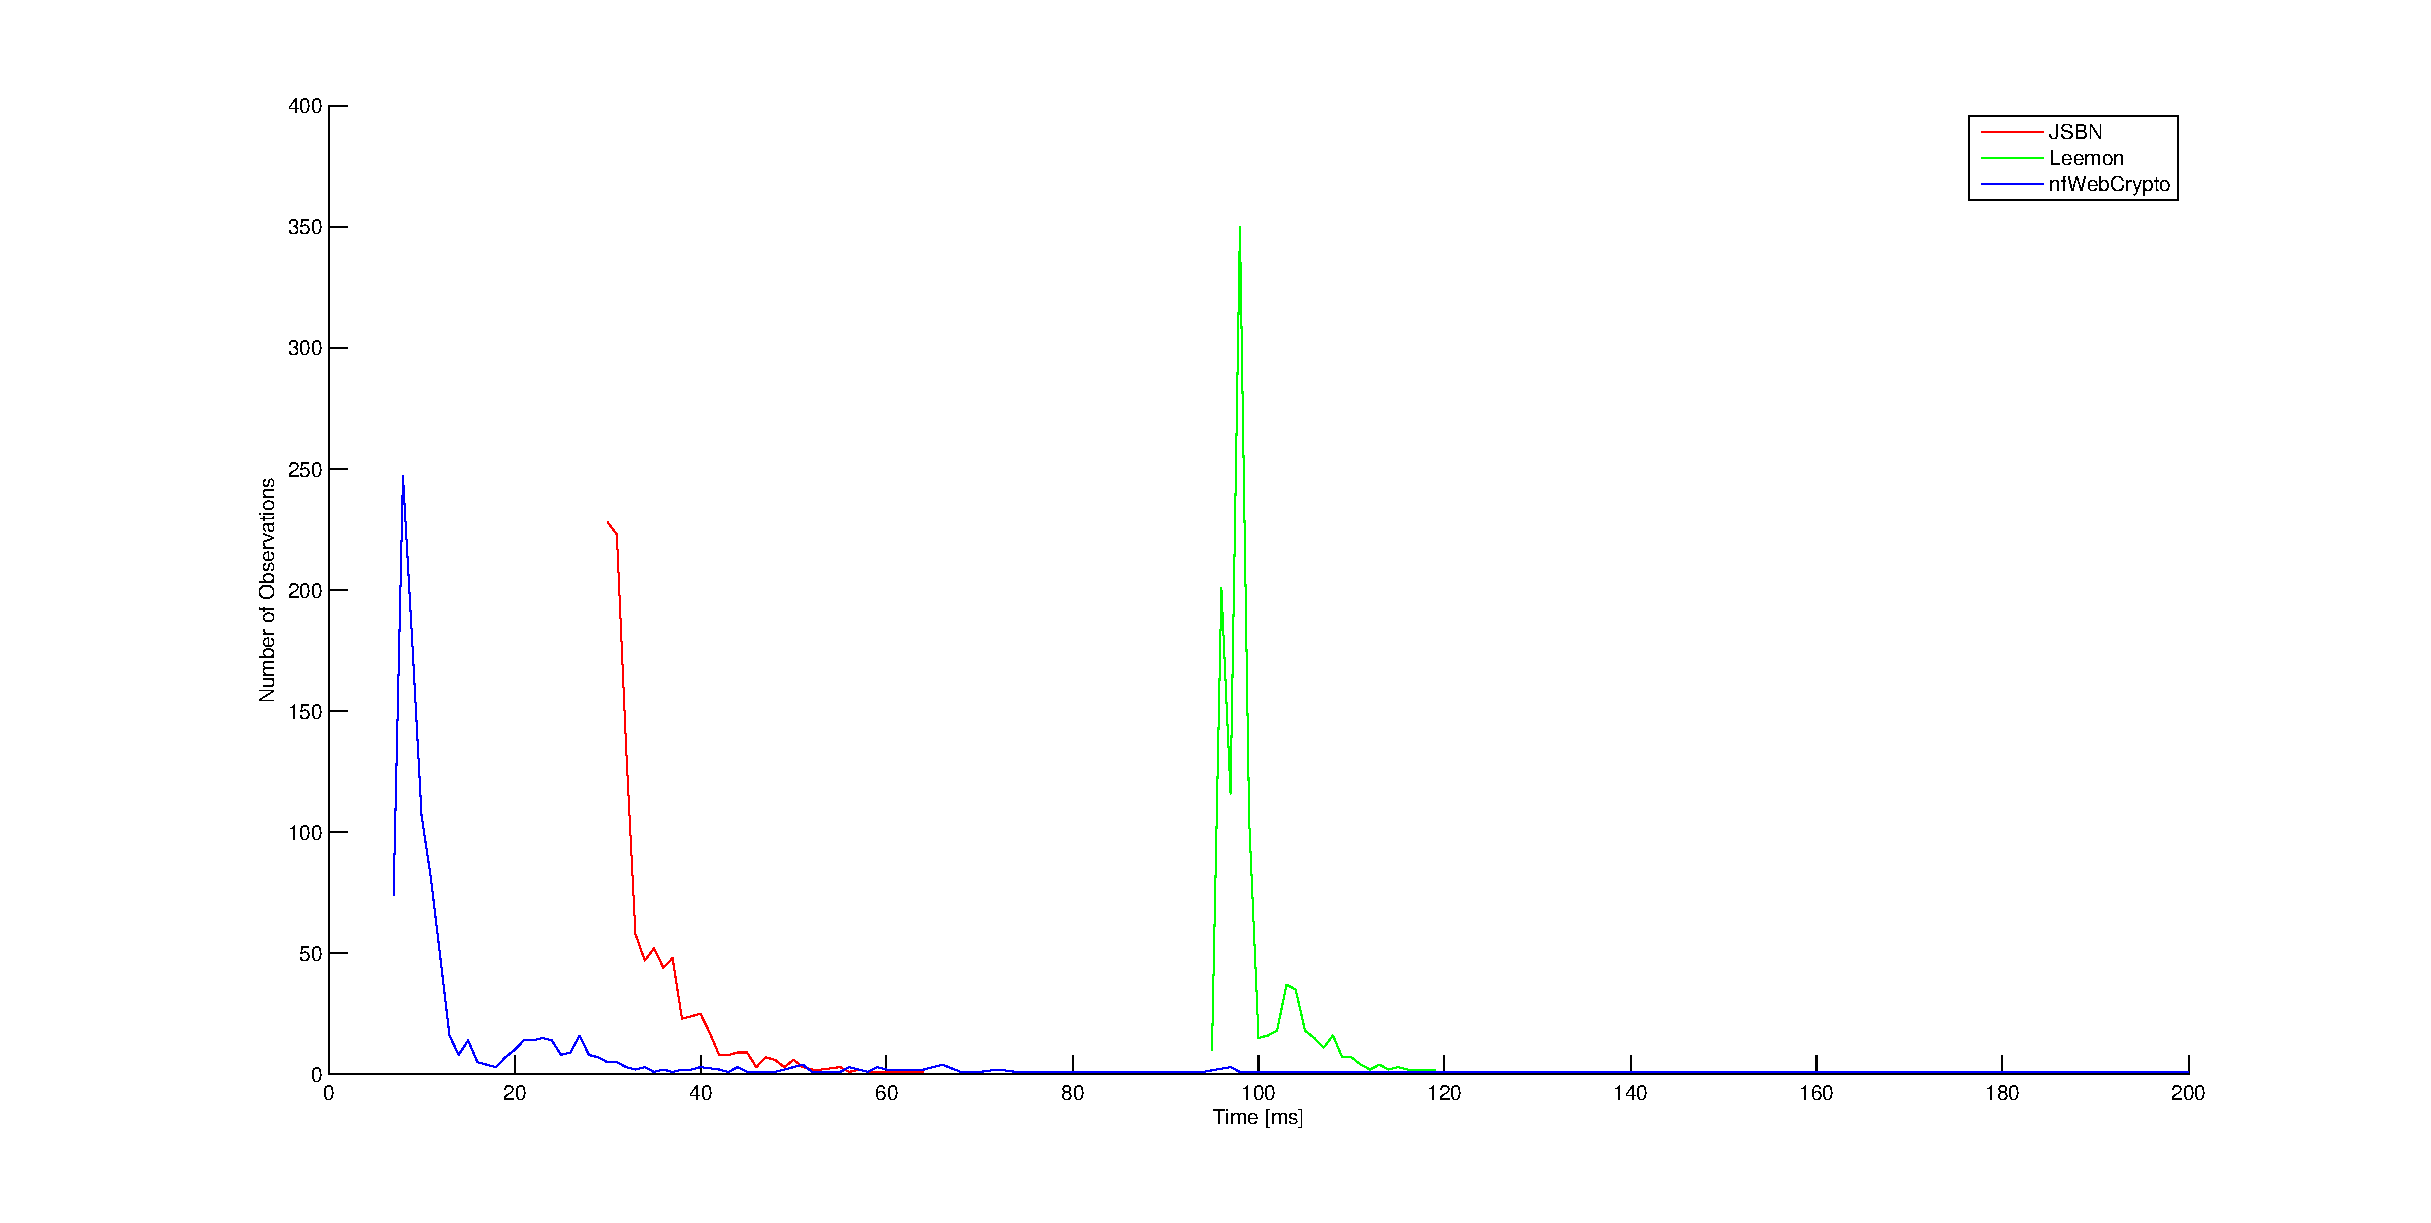
\includegraphics[width=\linewidth]{wc/modular_exponentiation.eps}}
  \caption{Modulaire exponentiatie}
  \label{fig:wc:modular_exponentiation}
\end{figure}

\begin{table}
  \begin{center}
    \begin{tabular}{r | c c}
      Library & Gemiddelde [ms] & Variantie [ms] \\ \hline
      JSBN & 33,9250 & 26,5019  \\
      Leemon & 99,1470 & 15,0785 \\
      NfWebCrypto & 16,0670 & 470,6251
    \end{tabular}
    \caption{Modulaire exponentiatie}
    \label{tab:wc:modular_exponentiation}
  \end{center}
\end{table}

\subsection{RSA}

Een tweede vergelijking werd gemaakt tussen JSBN en NfWebCrypto voor een RSA encryptie. Dit wordt niet gebruikt in Helios, maar ook deze resultaten zijn zeer interessant. De berekening van de RSA cijfertekst is opnieuw een modulaire exponentiatie (\ref{eq:wc:rsa}).\cite{rivest_shamir_adleman_rsa}

\begin{equation}
  \label{eq:wc:rsa}
  c = m^e \mod{n}
\end{equation}

\npar Hier is het paar $(n, e)$ de publieke sleutel van de partij waarvoor het bericht ge\"encrypteerd wordt. Voor de publieke exponent $e$ werd de standaardwaarde \np{65537} genomen. Merk op dat deze heel wat korter is dan de \np{1024}-bit exponenten die in de tests van \ref{sec:wc:modulaire_exponentiatie} gebruikt werden. De lengte van de modulus is \np{1024} bit.

\npar De JSBN library voorziet in enkele klassen specifiek voor RSA encryptie en decryptie. Het is dus zeer eenvoudig om een bepaalde klaartekst te encrypteren met een gegeven publieke sleutel. De Web Cryptography API ondersteunt hier het \texttt{RSAES-PKCS1-v1\_5} algoritme voor.\cite{rfc3447} Hoewel het mogelijk zou moeten zijn om publieke sleutels in het \texttt{SPKI}-formaat te importeren, bleek het opnieuw moeilijk om de sleutel die gebruikt werd voor de JSBN encryptie om te zetten. Daarom werd besloten om voor elke encryptie een nieuwe sleutel te genereren. De tijd die hiervoor nodig is, wordt niet meegerekend in het eindresultaat.

\npar Ook hier werd de encryptie \np{1000} keer uitgevoerd. De resultaten van deze test zijn terug te vinden in \ref{fig:wc:rsa} en \ref{tab:wc:rsa}. We zien dat de JavaScript implementatie voor deze veel kortere exponent sneller is dan de berekening door de NfWebCrypto plugin. De communicatie met de plugin weegt hier duidelijk zwaarder door.

\begin{figure}
  \center{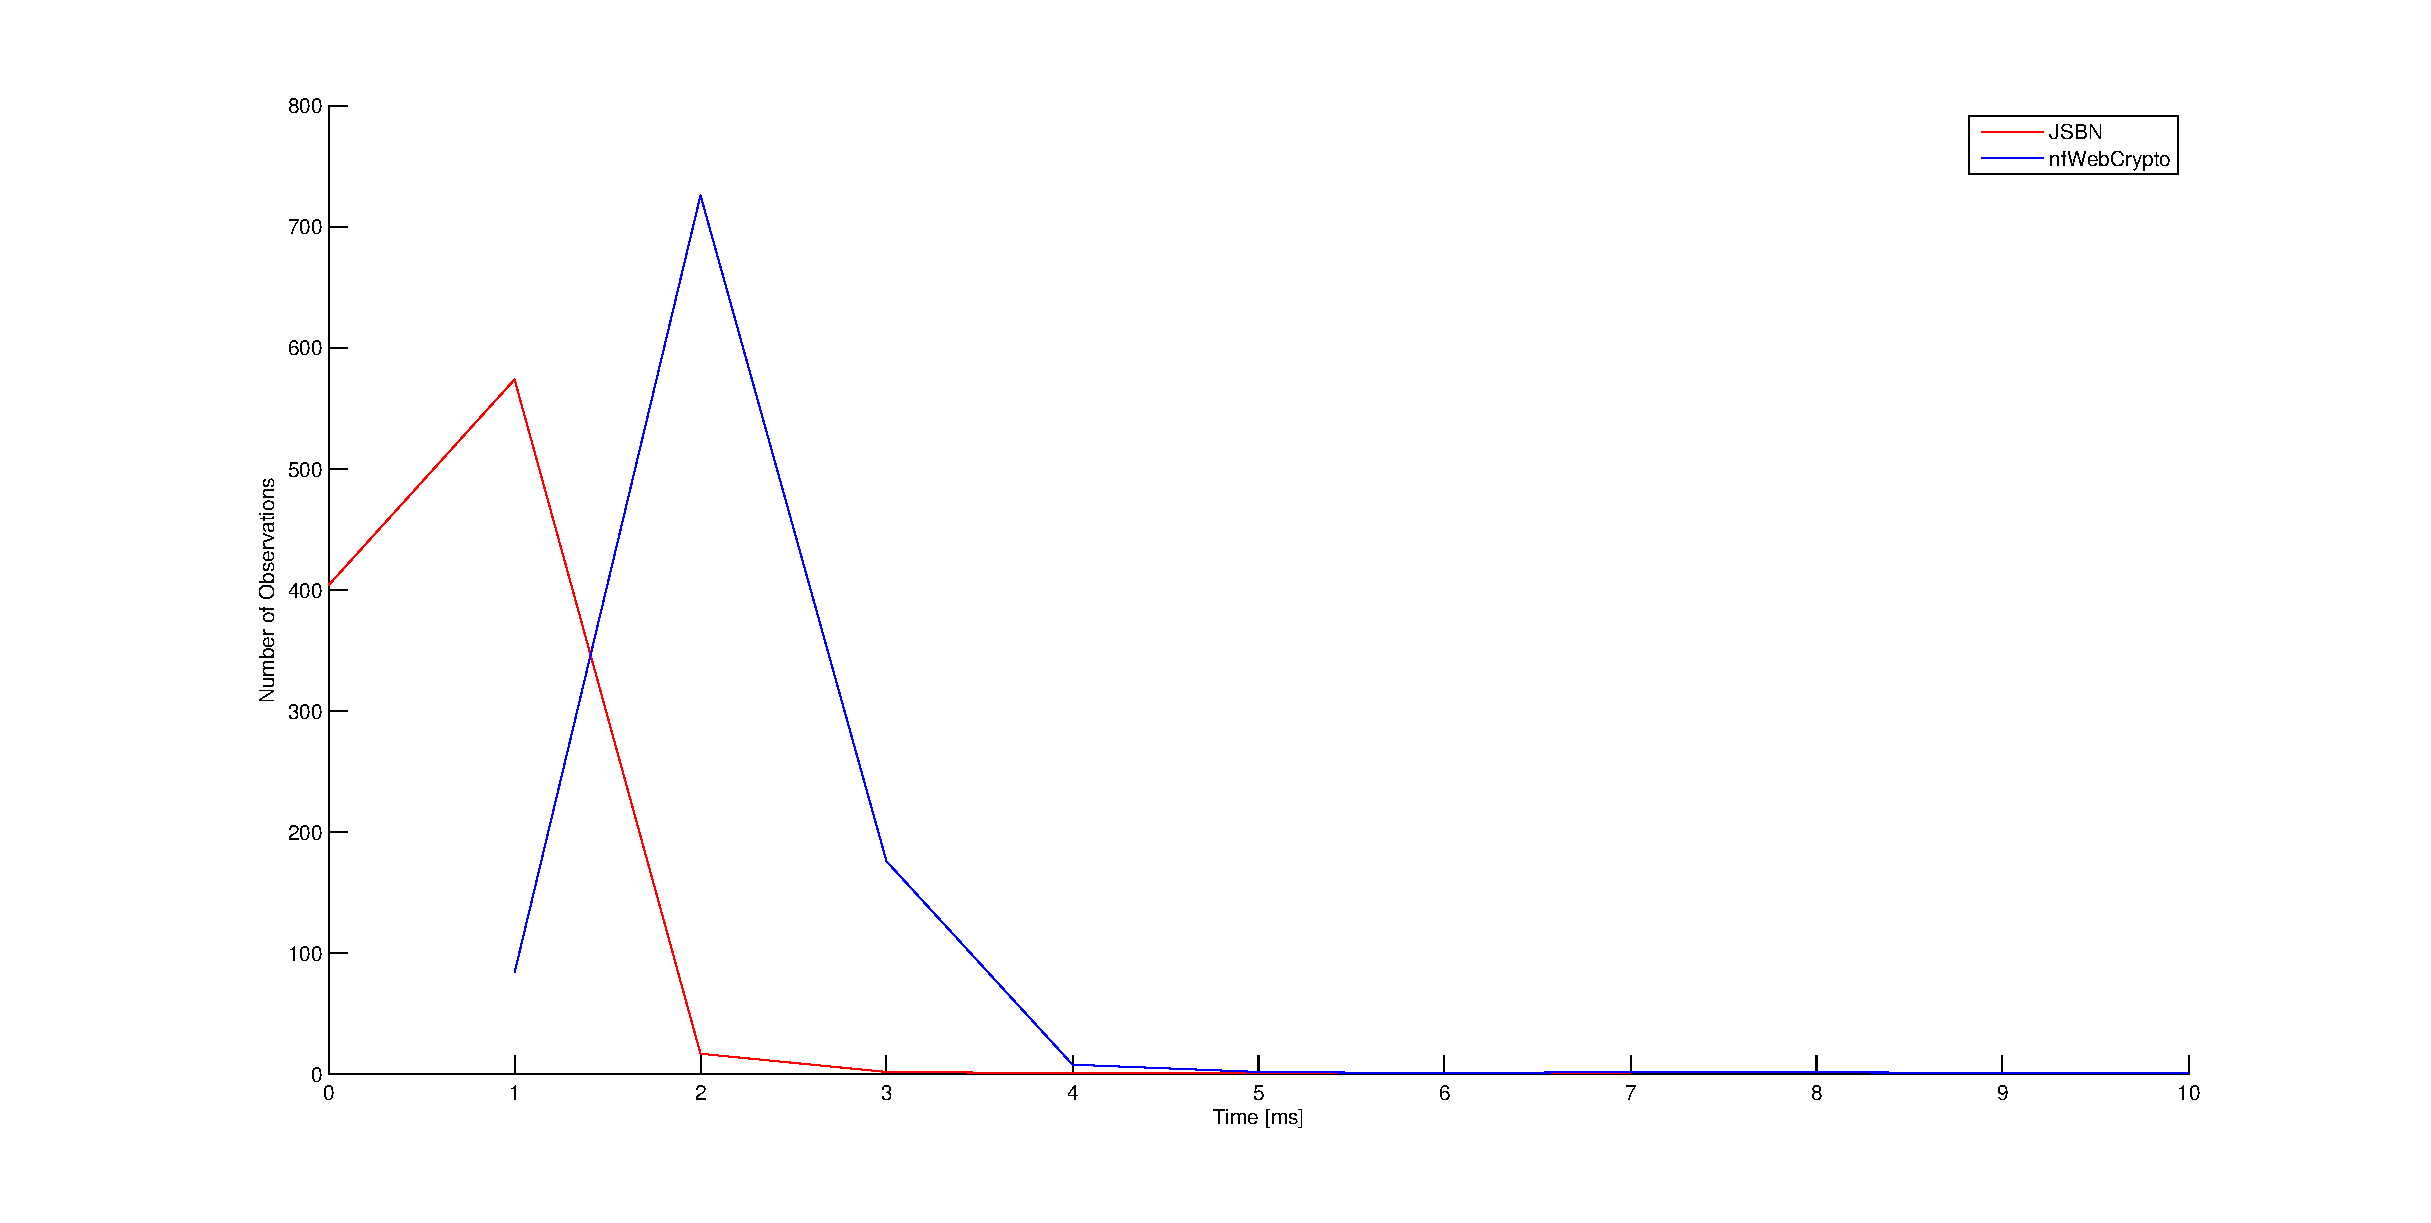
\includegraphics[width=\linewidth]{wc/rsa.eps}}
  \caption{RSA}
  \label{fig:wc:rsa}
\end{figure}

\begin{table}
  \begin{center}
    \begin{tabular}{r | c c}
      Library & Gemiddelde [ms] & Variantie [ms] \\ \hline
      JSBN & 0,6310 & 0,3632  \\
      NfWebCrypto & 2,1360 & 0,4219
    \end{tabular}
    \caption{RSA}
    \label{tab:wc:rsa}
  \end{center}
\end{table}

\section{Besluit}

Dankzij de Web Cryptography API zal het eenvoudiger worden om cryptografie te gebruiken in de browser. Bovendien is er een merkbare snelheidswinst ten opzichte van de huidige JavaScript implementaties, wat belangrijk is voor de gebruiksvriendelijk. 

\npar Dat slechts een beperkt aantal algoritmes ondersteund wordt, is een belangrijk nadeel van de API. Omdat de methodes die publiek beschikbaar zijn op een hoog niveau werken, is het zeer moeilijk om deze te gebruiken voor het versnellen van alternatieve algoritmes.

\npar Daarnaast was het ook ingewikkeld om sleutels die buiten de plugin gegenereerd waren, correct te importeren. Dit werd echter voornamelijk veroorzaakt door de encoding van de communicatie en is dus niet noodzakelijk een inherent probleem van de API.
